\chapter{Problem Background}

In this chapter we will analyze what were the already existing systems and tools we found interesting when we started our project.

\section{The problem}
The goal of this semester project is to unravel the emotion pattern underlying the sequences of songs in a playlist using automatic approaches of Emotion Detection on the lyrics.\par
The problem can be divided into two main parts:
\begin{enumerate}
\item Classify emotions of songs based their lyrics
\item Analyze emotion patterns in the playlists
\end{enumerate}

\section{Related work}
Emotion detection domain has already attracted many researchers from computer science, psychology, cognitive science and so on. \par
Before building our own emotion detection system we started by analyzing some of the already existent classifiers. \par
\paragraph{IBM Watson Natural Language Understanding}\cite{ibm_watson}
Watson is a question answering computer system capable of answering questions posed in natural language, developed by IBM.\par
Natural Language Understanding is a collection of APIs that allows to:
\begin{itemize}
\item Recognize the overall sentiment, in a scale from negative to positive [-1, 1];
\item Detect the emotion percentage between: joy, anger, disgust, sadness, fear;
\item Determine keywords ranked by relevance;
\item Extract entities: people, companies, organizations, cities and other information;
\item Classify content into hierarchical categories;
\item Identify general concepts that may not be directly referenced in the text; 
\end{itemize}

An example of IBM Watson NLU output is shown in figure \ref{fig:ibm_watson_wonderwall}.

\begin{figure}[H]
\centering
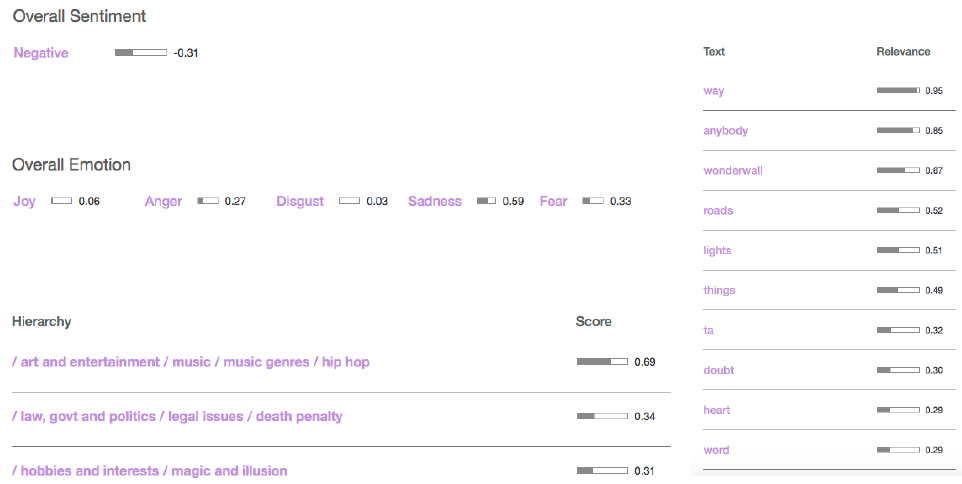
\includegraphics[width=1\textwidth]{./chapters/chapter3/images/ibm-watson-wonderwall}
\caption{IBM Watson Natural Language Understanding output while analyzing the lyric of Wonderwall, by Oasis}
\label{fig:ibm_watson_wonderwall}
\end{figure}

\paragraph{IBM Watson Tone Analyzer}\cite{ibm_watson_tone}
It uses linguistic analysis to detect joy, fear, sadness, anger, analytical, confident, and tentative tones found in text. It allows to select different sources: tweets, online reviews, email messages, or other text. It uses both:
\begin{itemize}
\item the document level: to get a sense of the overall tone;
\item the sentence level: to identify specific areas where tones are the strongest.
\end{itemize}

\paragraph{ParallelDots API}\cite{paralleldots}
It uses an Emotion Analysis classifier trained on a proprietary dataset and tells whether the underlying emotion behind a message is: Happy,
Sad, Angry, Fearful, Excited, Funny or Sarcastic. An example of its output is shown in figure \ref{fig:paralleldots}.

\begin{figure}[H]
\centering
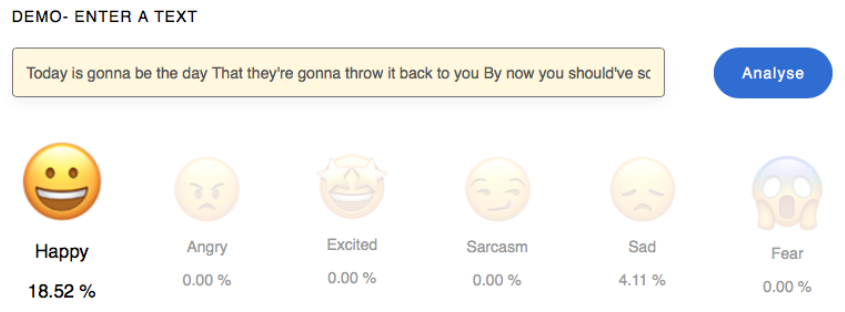
\includegraphics[width=0.9\textwidth]{./chapters/chapter3/images/paralleldots}
\caption{ParallelDots API applied on the lyrics of Wonderwall, from Oasis}
\label{fig:paralleldots}
\end{figure}

The results obtained with ParallelDots API and IBM Watson are quite different. Moreover we should consider that we don't know how the two tools internally parse the lyrics, i.e. how they do consider line breaks, line breaks without commas, etc. 

\paragraph{QEmotion}\cite{qemotion}
Qemotion detects the main emotion of the speech and define the corresponding emotion in terms of temperature:
\begin{itemize}
\item From $31^{\circ}$ to $40^{\circ}$ $\to$ Happiness
\item From $21^{\circ}$ to $30^{\circ}$ $\to$ Surprise
\item From $11^{\circ}$ to $20^{\circ}$ $\to $ Calm
\item From $6^{\circ}$ to $10^{\circ}$ $\to $ Fear
\item From $-5^{\circ}$ to $5^{\circ}$ $\to $ Sadness
\item From $-14^{\circ}$ to $-6^{\circ}$ $\to $ Anger
\item From $-20^{\circ}$ to $-15^{\circ}$ $\to $ Disgust
\end{itemize}

\section{NLP libraries}
In order to select the best Natural Language Processing library for our purpose we also analyzed pros and cons of the main Natural Language Processing libraries available, i.e. NLTK, TextBlob, Standord's CoreNLP and SpaCy. 

\paragraph{NLTK: Natural Language Toolkit}
NLTK is a leading platform for building programs to work with human language data. It provides easy-to-use interfaces to over 50 corpora and lexical resources, along with a suite of text processing libraries for classification, tokenization, stemming, tagging, parsing, and semantic reasoning and wrappers for industrial-strength NLP libraries\cite{nltk}. It is recommended only as an education and research tool. \\
Pros:
\begin{itemize}
\item its modularized structure makes it excellent for learning and exploring NLP concepts; 
\item over 50 corpora and lexicons, 9 stemmers, and a dozens of algorithms to choose from (this can also be considered as a con).
\end{itemize}
Cons: 
\begin{itemize}
\item Heavy library with a steep learning curve;
\item Slow and not production-ready. 
\end{itemize}

\paragraph{TextBlob}
Built on top on NLTK\cite{textblob}.\\
Pros: 
\begin{itemize}
\item More intuitive; 
\item Gentle learning curve. 
\end{itemize} 

\paragraph{Stanford's CoreNLP}
Stanford CoreNLP provides a set of human language technology tools. It can give the base forms of words, their parts of speech, whether they are names of companies, people, etc., normalize dates, times, and numeric quantities, mark up the structure of sentences in terms of phrases and syntactic dependencies, indicate which noun phrases refer to the same entities, indicate sentiment, extract particular or open-class relations between entity mentions, get the quotes people said, etc.\cite{stanfordcorenlp} It is a Java library with Python wrappers. \\
Pros:
\begin{itemize}
\item fast;
\item support for several major languages. 
\end{itemize}

\paragraph{SpaCy}
It is a new NLP library designed to be fast, streamlined and production-ready\cite{spacy}.\\
Pros:
\begin{itemize}
\item minimal number of options;
\item its philosophy is to only present the best algorithm for each purpose. 
\end{itemize}
Cons:
\begin{itemize}
\item it is new, so its support community is not as large as other libraries, but it is growing very fast.
\end{itemize}


\section{Word embedding techniques}
Word embeddings are a set of feature learning techniques mapping words or phrases from the vocabulary to vectors of real numbers. \par
These techniques map sparse word vectors into continuous space based on the surrounding context. For example if \textit{``salt''} and \textit{``seasoning''} appear within the same context, the model will indicate that \textit{``salt''} is conceptually closer to \textit{``seasoning''}, than another word, say \textit{``chair''}.\par
There are three main embedding techniques: Word2vec\cite{word2vec}, GloVe\cite{glove} and FastText\cite{fasttext}. 

The first two approaches treat each word in corpus like an atomic entity generating a vector for each of them. Specifically, word2vec tries to learn a vector representation of word occurring in similar contexts by using feedforward neural networks. On the other hand, GloVe, is a count-based model, which means that it firstly constructs a large co-occurrence matrix for the terms it finds, and then it factorizes (reduces the dimensionality) of this matrix to obtain fixed size vectors.

FastText, instead, treats each word as composed of character ngrams, so the vector for a word is made of the sum of this character n-grams\cite{fasttext}. \par
For example, for FastText,  the word vector for \textit{``apple''} is a sum of the vectors of the n-grams ``ap'', ``app'', ``appl'', ``apple'', ``ppl', ``pple'', ``ple'', ``le'' assuming 3 and 6 as minimum and maximum ngrams size.\\
The difference between Word2vec/GloVe and FastText manifests as follows:
\begin{enumerate}
\item \textit{Rare words}: even if words are rare, their character n-grams are still shared with other words - hence the embeddings with FastText can still be good;
\item \textit{Out of vocabulary words}: FastText can construct the vector for a word from its character n-grams even if word does not appear in training corpus;
\item \textit{Hyperparameters choice}: FastText requires to  choose the minimum and maximum n-grams sizes, and this directly impacts the computation time and the memory requirements. 
\end{enumerate}

\section{Tools Choice}

Given the considerations expressed above, for our project we decided to use SpaCy and an already trained language model provided by the same developers, built using GloVe.

SpaCy was choosen among the other analyzed libraries for its efficiency and for its simplicity. 

Regarding the word embedding tool of choice, GloVe was firstly choosen because we did not believe that we needed all the complications introduced in FastText. However, we decided to give FastText a try but we got worse results, confirming our intuition. Specifically we tried to featurize our dataset (this process is later explained in more details) both using FastText and GloVe and, in average, we always obtained slightly worse accuracy performances while using FastText-based featurization.

Therefore we decided to stick with GloVe. Specifically, the language model we used provides 685k unique 300-dimensional word embedding vectors, which were trained on natural language text coming from OntoNotes 5\cite{ontonotes5} and Common Crawl\cite{common-crawl}.